% GENERATED BY sshrc_figures.py - edit that file, not this one.
% The document that inputs this file supplies the float, the caption and the label.
% Stream B. Committees, left to right within each year: Economics, Business (14A, 14B, 14C), Multidisciplinary humanities, Multidisciplinary social sciences (23, 23A, 23B).
\definecolor{sshrcA}{HTML}{2A78D6}
\definecolor{sshrcB}{HTML}{EB6834}
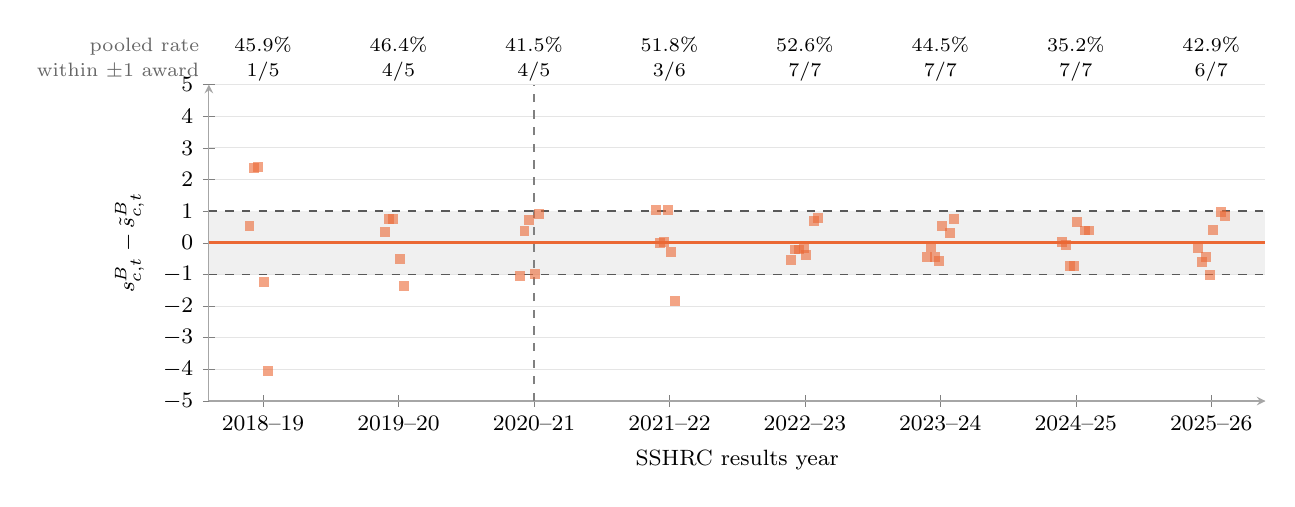
\begin{tikzpicture}
\begin{axis}[
  width=15cm, height=5.6cm,
  xmin=2017.6, xmax=2025.4, ymin=-5, ymax=5,
  xtick={2018,2019,2020,2021,2022,2023,2024,2025}, xticklabels={2018--19,2019--20,2020--21,2021--22,2022--23,2023--24,2024--25,2025--26},
  axis x line=bottom, axis y line=left, axis line style={gray!70},
  ymajorgrids, grid style={gray!20},
  tick label style={font=\footnotesize}, label style={font=\footnotesize},
  xlabel={SSHRC results year}, ylabel={$s^{B}_{c,t}-\tilde{s}^{B}_{c,t}$}, ylabel style={align=center},
  clip=false,
  ytick distance=1,
]
\fill[gray!12] (axis cs:2017.6,-1) rectangle (axis cs:2025.4,1);
\draw[gray, dashed, line width=0.7pt] (axis cs:2020,-5) -- (axis cs:2020,5);
\addplot[color=sshrcB, line width=1.2pt, forget plot, domain=2017.6:2025.4, samples=2] {0};
\addplot[gray!70!black, line width=0.7pt, dashed, forget plot, domain=2017.6:2025.4, samples=2] {-1};
\addplot[gray!70!black, line width=0.7pt, dashed, forget plot, domain=2017.6:2025.4, samples=2] {1};
\addplot[only marks, mark=square*, mark size=1.8pt, color=sshrcB,
  mark options={fill opacity=0.6, draw opacity=0}]
  coordinates {(2017.93,2.36) (2017.96,2.41) (2017.90,0.54) (2018.01,-1.25) (2018.04,-4.06) (2018.93,0.76) (2018.96,0.76) (2018.90,0.33) (2019.01,-0.50) (2019.04,-1.35) (2019.90,-1.05) (2019.93,0.38) (2019.96,0.72) (2020.01,-0.97) (2020.04,0.91) (2020.90,1.04) (2020.93,0.01) (2020.96,0.04) (2020.99,1.04) (2021.01,-0.29) (2021.04,-1.84) (2021.90,-0.53) (2021.93,-0.21) (2021.96,-0.21) (2021.99,-0.16) (2022.01,-0.37) (2022.07,0.68) (2022.10,0.79) (2022.90,-0.46) (2022.93,-0.13) (2022.96,-0.46) (2022.99,-0.57) (2023.01,0.54) (2023.07,0.31) (2023.10,0.76) (2023.90,0.04) (2023.93,-0.07) (2023.96,-0.72) (2023.99,-0.72) (2024.01,0.67) (2024.07,0.39) (2024.10,0.39) (2024.90,-0.16) (2024.93,-0.60) (2024.96,-0.45) (2024.99,-1.02) (2025.01,0.42) (2025.07,0.98) (2025.10,0.84)};
\node[font=\scriptsize, anchor=base east, text=gray!80!black] at ([yshift=12pt]axis cs:2017.6,5) {pooled rate};
\node[font=\scriptsize, anchor=base] at ([yshift=12pt]axis cs:2018,5) {45.9\%};
\node[font=\scriptsize, anchor=base] at ([yshift=12pt]axis cs:2019,5) {46.4\%};
\node[font=\scriptsize, anchor=base] at ([yshift=12pt]axis cs:2020,5) {41.5\%};
\node[font=\scriptsize, anchor=base] at ([yshift=12pt]axis cs:2021,5) {51.8\%};
\node[font=\scriptsize, anchor=base] at ([yshift=12pt]axis cs:2022,5) {52.6\%};
\node[font=\scriptsize, anchor=base] at ([yshift=12pt]axis cs:2023,5) {44.5\%};
\node[font=\scriptsize, anchor=base] at ([yshift=12pt]axis cs:2024,5) {35.2\%};
\node[font=\scriptsize, anchor=base] at ([yshift=12pt]axis cs:2025,5) {42.9\%};
\node[font=\scriptsize, anchor=base east, text=gray!80!black] at ([yshift=3pt]axis cs:2017.6,5) {within $\pm1$ award};
\node[font=\scriptsize, anchor=base] at ([yshift=3pt]axis cs:2018,5) {1/5};
\node[font=\scriptsize, anchor=base] at ([yshift=3pt]axis cs:2019,5) {4/5};
\node[font=\scriptsize, anchor=base] at ([yshift=3pt]axis cs:2020,5) {4/5};
\node[font=\scriptsize, anchor=base] at ([yshift=3pt]axis cs:2021,5) {3/6};
\node[font=\scriptsize, anchor=base] at ([yshift=3pt]axis cs:2022,5) {7/7};
\node[font=\scriptsize, anchor=base] at ([yshift=3pt]axis cs:2023,5) {7/7};
\node[font=\scriptsize, anchor=base] at ([yshift=3pt]axis cs:2024,5) {7/7};
\node[font=\scriptsize, anchor=base] at ([yshift=3pt]axis cs:2025,5) {6/7};
\end{axis}
\end{tikzpicture}
